% -*- fill-column: 80; -*-
\documentclass[acmsmall,screen,nonacm]{acmart}
\usepackage{mathpartir}
\usepackage{tikz-cd}
\usepackage{lipsum}
\usepackage{enumitem}
\usepackage{wrapfig}
\usepackage{fancyvrb}
\usepackage{hyperref}
\usepackage{cleveref}
\usepackage{stmaryrd}
\usepackage{tikz}
\usetikzlibrary{automata, positioning, arrows, fit}

\usepackage{pdfpages}

\usepackage{todonotes}

\newcommand{\sem}[1]{\llbracket{#1}\rrbracket}
\newcommand{\cat}[1]{\mathbf{#1}}
\newcommand{\lto}{\multimap}
\newcommand{\tol}{\mathrel{\rotatebox[origin=c]{180}{$\lto$}}}
\newcommand{\String}{\Sigma^{*}}
\newcommand{\Set}{\mathbf{Set}}
\newcommand{\Gr}{\mathbf{Gr}}
\newcommand{\Type}{\mathbf{Type}}
\newcommand{\Prop}{\mathbf{Prop}}
\newcommand{\Bool}{\mathbf{Bool}}
\newcommand{\nat}{\mathbb{N}}

\newcommand{\gluedNL}{{\mathcal G}_S}
\newcommand{\gluedNLUniv}{{\mathcal G}_{S,i}}
\newcommand{\gluedL}{{\mathcal G}_L}

\newcommand{\simulsubst}[2]{#1\{#2\}}
\newcommand{\subst}[3]{\simulsubst {#1} {#2/#3}}
\newcommand{\letin}[3]{\mathsf{let}\, #1 = #2 \, \mathsf{in}\, #3}
\newcommand{\lamb}[2]{\lambda #1.\, #2}
\newcommand{\lamblto}[2]{\lambda^{{\lto}} #1.\, #2}
\newcommand{\lambtol}[2]{\lambda^{{\tol}} #1.\, #2}
\newcommand{\dlamb}[2]{\overline{\lambda} #1.\, #2}
\newcommand{\app}[2]{#1 \, #2}
\newcommand{\applto}[2]{#1 \mathop{{}^{\lto}} #2}
\newcommand{\apptol}[2]{#1 \mathop{{}^{\tol}} #2}
\newcommand{\PiTy}[3]{\Pi #1 : #2.\, #3}
\newcommand{\SigTy}[3]{\Sigma #1 : #2.\, #3}
\newcommand{\LinPiTy}[3]{\widebar\Pi #1 : #2.\, #3}
\newcommand{\LinSigTy}[3]{\widebar\Sigma #1 : #2.\, #3}
\newcommand{\amp}{\mathrel{\&}}
\newcommand{\GrTy}{\mathsf{Gr}}

\newcommand{\ctxwff}[1]{#1 \,\, \mathsf{ok}}
\newcommand{\ctxwffjdg}[2]{#1 \vdash #2 \,\, \mathsf{type}}
\newcommand{\linctxwff}[2]{#1 \vdash #2 \,\, \mathsf{ok}}
\newcommand{\linctxwffjdg}[2]{#1 \vdash #2 \,\, \mathsf{linear}}

\newif\ifdraft
\drafttrue
\newcommand{\steven}[1]{\ifdraft{\color{orange}[{\bf Steven says}: #1]}\fi}
\renewcommand{\max}[1]{\ifdraft{\color{blue}[{\bf Max says}: #1]}\fi}
\newcommand{\pedro}[1]{\ifdraft{\color{red}[{\bf Pedro says}: #1]}\fi}
\newcommand{\pipe}{\,|\,}

\newcommand{\todoin}[1]{\ifdraft{\todo[inline]{TODO:\@ #1}}\fi}

\begin{document}

\pagestyle{plain}

\includepdf{cover.pdf}

\pagebreak

\ifdraft{
\listoftodos{list of todos}
\pagebreak}\fi

\title{Formal Grammars as Types in Non-commutative Linear-Non-Linear Type Theory}

\author{Steven Schaefer}
\affiliation{\department{Electrical Engineering and Computer Science}
  \institution{University of Michigan}
  \country{USA}
}
\email{stschaef@umich.edu}

\author{Max S. New}
\affiliation{
  \department{Electrical Engineering and Computer Science}
  \institution{University of Michigan}
  \country{USA}
}
\email{maxsnew@umich.edu}

\author{Pedro H. Azevedo de Amorim}
\affiliation{
  \department{Department of Computer Science}
  \institution{University of Oxford}
  \country{UK}
}
\email{pedro.azevedo.de.amorim@cs.ox.ac.uk}

\makeatletter
\let\@authorsaddresses\@empty
\makeatother

\begin{abstract}
  In this paper, we give a type system in which we can
  internally carry out many classical constructions from
  the theory of formal grammars. Inspired by the common
  structure underlying various ideas in formal language
  theory, our type theory makes these relationships explicit
  and provides a unifying syntax to reason about formal
  grammars. We discuss application to the design and
  implementation of correct-by-construction parsers for use
  in real-world compilers.
\end{abstract}

\maketitle

\setcounter{page}{1}

\section{Introduction}
% idk some intro about verification in general, then build up to verifying compilers, and ultimately parsers
In the realm of software development, ensuring the correctness and reliability
of code is of the utmost importance. In practice, developers often write tests
to gain confidence that they have written a program correctly; however,
program correctness cannot be guaranteed through testing alone. Where testing is
incomplete, we may further use formal methods for generating mathematical proofs of
correctness for our software.

Importantly, any proof of correctness is relative to the formal specification given
for the program. For instance, even if one provides a verified artifact for
their system's source code, it is not a guarantee that this system will run as
expected on real machines because it is not taking into account hardware
semantics.
The developer puts a large degree of implicit trust in
their compiler to generate a binary that reflects the intended behavior of their
source code. To bridge this gap, the compilers themselves may be verified, such
as CompCert\cite{leroy_formal_2009} --- a verified C compiler ---
and CakeML\cite{kumar_cakeml_2014} --- a verified implementation of an ML-like language.

Unfortunately even the apparent assurances associated with
this verification were not enough, as even early versions of CompCert still
had bugs\cite{yangFindingUnderstandingBugs}. Despite significant effort
verifying the middle- and backends of their C compiler, Leroy et al.\ did not
initially prove the correctness of their compiler frontend. When considering
machine traces, the presence of
these parsing bugs can jeopardize the guarantees provided by other verification
efforts. That is, verification exists on a stack of trust, and even one break in
the chain of verification can lead to incorrect behavior of real machines.

Several years after its release, the CompCert project was later updated to use a
verified parser\cite{jourdanValidatingLRParsers2012}. This parser was generated
by Menhir --- an LR parser generator --- and verified
post-hoc. After-the-fact
verification efforts like this are
time-intensive and difficult to generalize. Significant person-hours are
invested in managing the idiosyncrasies of the parser-generator being used and
even the particular grammar describing the
language.

To aid in the development of verified parsers, the primary contribution
of this paper is
an type
theory whose types natively capture the semantics of formal
grammars. Types in this theory are grammars, and terms are
parse transformers. This kind of type theory naturally
requires (non-commutative) linear and dependent types.
Within this formalism, we may define parsers as terms
defined in the context of an input string. Moreover, by virtue of
typechecking, these parsers are \emph{correct-by-construction}. The intrinsic
verification gained from the type system therefore removes the need for a
post-hoc verification in a language like Coq, thus lowering the barrier to
compiler frontend verification.

Substructural logics, like linear and separation logic, offer precise control
over how values from a type may be used, in particular how many times a value
may be used in a derivation. This control enables \emph{resource-sensitive}
reasoning, where we may treat a resource as \emph{consumed} after usage. In the
context of parsing, we may treat the characters composing a string as finite resources
that are consumed at parse-time.

Dependent type theory extends the simply-typed $\lambda$-calculus by allowing type
definitions to contain the occurrence of a term. In lieu of set-based
foundations, this extension can then be taken as a foundation for mathematics.
The expressive power unlocked by this insight has enabled the development of
dependently-typed proof assistants
such as Coq or Agda. Within each of these languages, systems may be given very
precise functional specifications of their behavior.

In 1995, Benton et al.
\cite{bentonMixedLinearNonlinear1995} first gave categorical models of a logic
that synthesized linear and non-linear logic. Later, Krishnaswami et al.
\cite{krishnaswami_integrating_2015} built upon this work to develop a type
system that unifies both linear and
dependent types --- referred to as a \emph{linear-non-linear} (LNL) type theory. In
such settings, we have two sub-theories --- one linear and one non-linear. The
linear sub-theory embeds ordinary linear types without dependence, while the
non-linear sub-theory embeds standard Martin-L\"of type theory. The interplay of
linear types with dependence lives at the boundary between these two fragments.
Benton et al.\ gives an accounting of how we may jump between these
fragments via a monoidal adjunction $F \dashv G$ between linear terms and
non-linear terms.

To the end of defining real verified
parsers, in our LNL theory we define a parser as a term,

\crefname{equation}{}{}
\begin{equation}
  \label{eq:parser}
  w : \String \vdash \mathsf{parse}_{g}(w) : g \oplus \top
\end{equation}

We will investigate the precise meaning of judgments like \cref{eq:parser} in
\cref{sec:tt}, but first let's get an intuitive feel for the meaning behind such a
term. On the left of the turnstile occurs a single string $w$, we may think of
this describing what resources are linearly available to us. Using each piece of
our the context on the left of the turnstile, we build a term
$\mathsf{parse}_{g}(w)$ of type $g \oplus \top$. Notably, the type being
instantiated is a sum type, and the data of which side we inject into denotes
whether the string is accepted or rejected by the parser. That is all to say, a
parser takes in an input string and either matches it to the desired grammar or
rejects the string.

Practical parsers are often implemented via an abstract automaton. For instance,
a parser may translate a grammar into a state machine recognizes the
same language as the original grammar, as the automata
point-of-view lends itself to straightforward execution. The
strength of our syntax is that it allows us to describe
these automata as grammars themselves. Moreover, the
equivalence between the grammar and automata presentations
is derivable as a proof term within the theory. This allows
us access to simultaneously internalization of the equivalence
between grammars and automata as well as the ability to
export to automaton implementations of a parser that are executable.

To realize an executable implementation of our type theory,
we shallowly embed it in Agda. Because our implementation is
defined as a function in Agda, we can leverage the Agda
ecosystem for code generation. Further, in lieu of
implementing a complete language from scratch, we make use of the
Agda proof system as a setting to guarantee correctness of
our generate parsers.

Within this paper, we give our progress in defining a verified
parser for regular expressions. The construction of such a parser entails
the definition of a parser for deterministic finite automata (DFA) grammars,
and an equivalence proof between DFAs and regular expressions. We have thus far
completed the construction of a parser for DFAs $D$,

\[
  w : \String \vdash \mathsf{parse}_{D}(w) : D \oplus \top
\]

and half of the equivalence proof between DFAs and regular expressions, both
formalized in Agda. Upon completion of the second half of this proof, we would
have a system where a user could simply give a regular grammar and then extract
an intrinsically verified parser for it. In future work, we
hope to show an analogous construction involving pushdown
automata (PDAs) and context-free grammars.

The contributions of this paper include an LNL theory for reasoning about formal
grammars, the encoding of automata as formal grammars in this theory, and the
definition of parser terms for DFA grammars. The contents include,

\begin{itemize}
  \item A syntax-independent definition of formal grammar
  \item The formal rules governing our type system
  \item Interpretations of the type system for reasoning about formal grammars
        and formal languages
  \item The presentation of automata as grammars
  \item The definition of a parser within our type system
\end{itemize}

\section{A Syntax-Independent Notion of Syntax}
\label{sec:synindsyn}

% \max{this section doesn't flow naturally from the intro, which is all about the
%   type theory and parsing. This is where you want to outline in the intro and
%   possibly say here that we want to revisit ``formal grammar theory'' and then
%   we will make a type theory that has formal grammar theory as its semantics.}

In this section we will revisit some foundational ideas in formal
grammar theory, before giving a type
theory for which formal grammars serves as its semantics.

Formal languages and grammars are among some of the oldest and most studied areas in
theoretical computer science. The developments of the 1950s and 1960s gave rise
to expressive formalism for reasoning about grammars, and further practical
algorithms for constructing parsers for regular and context-free grammars.

A grammar $G$ is often described generatively as a set of production rules for
generating strings. Often this is presented as a finite set of nonterminal
symbols $N$, a finite set of terminal symbols $\Sigma$, and a finite set of rewriting
rules for substitution of nonterminals. In this setting, we continually apply
rewrite rules until we are left only with a string of terminals
$w \in \String$. We will give a more precise notion of
grammar in a moment, but for now let us take this intuitive view of grammars as
string generators.

One of the primary objects of study is that of a \emph{formal language} over
a fixed alphabet $\Sigma$. A language $L$ is a \emph{subset} of strings
$L \subseteq \String$. This notion of formal language gives an intuitive
set-based semantics for grammars. That is, we may interpret a grammar $G$ as the
language $L(G)$ that is generated by it. We are yet to give any precise
definition of what we mean by ``grammar'', although we note that any suitable
notion of grammar can be given a language semantics as above.

Formal languages serve as a basis for mathematically specifying a
\emph{recognizer} --- a
function $r : \String \to \Bool$ that determines if a string belongs to a
given language. However, they are insufficient for specifying a \emph{parser}
--- a function that decomposes a string into semantic components that adhere to
the structure of a formal grammar. In practice, parsers don't just tell you
if a string is valid or invalid. Instead, they emit structured data such as
abstract syntax trees (ASTs).

This motivates our first conceptual contribution, a simple and
syntax-independent notion of formal grammar:

\begin{definition}
  \label{def:grammar}
  A \emph{formal grammar} $G$ over a fixed alphabet $\Sigma$ is a function
  $G : \String \to \Set$.
\end{definition}

We say that a grammar $G$ associates to every string $w$ the set\footnote{We
  make little comment as to which foundations we use to encode sets. We argue\max{drop ``We argue''}
  that our construction is agnostic to the particular foundation, and so without
  loss of generality\max{incorrect use of ``without loss of generality''} we may take a class of small sets, a Grothendieck universe,
  a type theoretic universe, or any similar foundation. Here we choose a type
  theoretic universe.} $G w$ of parse
trees showing that $w$ matches $G$.

The simplest class of formal grammar on the Chomsky\max{first mention of Chomsky hierarchy, why not bring it up earlier when you are describing what a grammar is? Also cite}
hierarchy are the \emph{regular expressions}

\max{inaccurate reflection of common terminology. These are regular expressions,
  regular grammars usually means a CFG with a restriction on recursion that
  ensures you only allow Kleene star.}.

\begin{gather*}
  \mathsf{Char} \in \Sigma \\
  \mathsf{Reg} ::= \mathsf{Char}~|~I~|~\mathsf{Reg} \otimes \mathsf{Reg}~|~\mathsf{Reg} \oplus \mathsf{Reg}~|~\mathsf{Reg}^{*}
\end{gather*}

Here, we use a non-standard syntax inspired by linear logic. Disjunction of
regular expressions is written $\oplus$, and concatenation of regular
expressions is written like the linear tensor product $\otimes$. The
empty grammar is sometimes written in the same manner as the empty string,
$\varepsilon$, but we instead choose to represent the empty grammar by $I$. This
is also linear logic syntax to represent the unit $I$ of the operation $\otimes$.

To see an illustration of the notion of grammar given in \cref{def:grammar}, consider the regular expression
$G = (a \otimes b)^{*} \otimes a$ --- a sequence of 0 or more $ab$'s followed by
an $a$. We may think of $G$ as a function that takes in strings and outputs all
of the parse trees of that string. Passing the input string $baa$ through $G$
would output the empty set, because there are no $G$-parses of $baa$. However,
passing $aba$ through $G$ would output a singleton set, as there is only a
single $G$-parse of $aba$. Namely, the one that breaks up $aba$ as $(ab)a$.

Observe that for any input string $w$ for the above grammar $G$, $G(w)$ is
either empty or a singleton set. Either the string isn't parsed by $G$,
or it is parsed by $G$ for exactly one reason. That is, $G$ is
\emph{unambiguous}. If we instead consider the grammar
$H = (a \otimes b)^{*} \oplus (b \otimes a)^{*}$ there are now ambiguities. For
instance, what is the action of $H$ on the empty string $\varepsilon$?
The empty string $\varepsilon$ matches both $(a \otimes b)^{*}$ and $(b \otimes a)^{*}$, so
$\varepsilon$ can match either the left or the right pattern
of $H$. As a result, $H(\varepsilon)$ is a two-element set.

For every grammar, we can specify a formal language recognized by that grammar. By ranging over all input strings, we can
see that every formal grammar $G$ induces a formal language $L_{G}$,

\[
  L_{G} = \{ w \in \String : G w \text{ is inhabited} \}
\]

As they are just sets, formal languages naturally are
endowed with a partial
order via the subset inclusion ordering. Similarly, formal grammars are
naturally endowed with the structure of a \emph{category} where a morphism
$f : G \to H$ is given by a \emph{family} of functions:


\[
  f^{w} : Gw \to Hw, w \in \String
\]

Intuitively, we read a morphism of grammars as a \emph{parse transformer}: $f$
translates a
$G$-parse of $w$ into an $H$-parse of $w$. The notion of isomorphism induced by
this categorical structure encodes that two grammars are equivalent if there is
a bijective translation of parses. Isomorphisms in the category of
grammars are precisely Chomsky's notion of \emph{strong equivalence} of
grammars \cite{chom1963}.

The category of grammars is quite rich in structure. It can
equivalently be described as the functor category $\Set^{\String}$, where
$\String$ is a discrete category. That is, the objects in $\String$ are strings
and the only morphisms are identity morphisms. Such functor categories into
$\Set$ --- often called presheaf categories --- carry a remarkable amount of
structure. In fact, any presheaf category naturally models dependent type
theory, which we exploit to motivate the design of the formalism
presented in \cref{sec:tt}.


\section{A Type Theory to Reason About Formal Grammars}
\label{sec:tt}

\subsection{Syntax}
\label{subsec:syntax}

In this section we will walk through most of the syntax of our type theory. We
include the full syntax in \cref{sec:infer}.

The linear typing judgment in our syntax takes on the following schematic form,
\[
  \Gamma ; \Delta \vdash M : A
\]

Let us briefly digest what this judgment is trying to say. First, $A$ represents
a \emph{linear type} in our syntax. The intended semantics of these linear types
are formal grammars. That is, the linear typing system is designed to syntactically
reflect the behavior of formal grammars. For this reason, we may often
interchangeably use the terms ``linear type'' and ``grammar''. To see the
correspondence between types and grammars, note that the constructors for linear types
mirror operations on formal grammars. For example, we have linear type constructors
$\otimes$, $\oplus$, and $\amp$ which correspond to grammar concatenation,
disjunction, and conjunction, respectively. The other type constructors also have
corresponding grammar intuition which may be seen in \cref{subsubsec:other}.

$M$ is an inhabitant of type $A$, which we want to think of as a parse tree of
the grammar $A$. The core idea of this entire paper follows precisely from this
single correspondence: grammars are types, and the inhabitants of these types
are parse trees for the grammars!

$\Gamma$ represents a \emph{non-linear context} --- also referred to as an
\emph{intuitionistic} context. The non-linear fragment of the theory
corresponds to usual Martin-L\"of type theory. That is, the intuitionistic
contexts obey all of the usual structural rules --- contraction, weakening, and
exchange --- so we may use their contents as many times as we'd like.

On the other hand $\Delta$ represents a \emph{linear context}. These linear
contexts
behave substructurally --- in particular they have no contraction, weakening, or exchange
rule. This means that everything within $\Delta$ must be used \emph{exactly
  once} and \emph{in order of occurrence}. Thus, we can think of the linear
contexts as an ordered list of limited
resources. Once a resource is consumed, we cannot make reference to it again.
We may then
think of the variables in a linear context akin to building blocks for
constructing patterns over strings.

In the realm of parsing, our substructural
restrictions make it so that the linear contexts behave quite similarly to
formal grammars. For instance, linear context extension mirrors concatenation of
grammars which may be seen via the introduction rule for $\otimes$,

\[
  \inferrule{\Gamma ; \Delta \vdash e : A \\ \Gamma ; \Delta' \vdash e' : B}{\Gamma ; \Delta , \Delta' \vdash e \otimes e' : A \otimes B}
\]

Just as two grammars may be concatenated, if we can build an $A$ with the
contents of $\Delta$, and a $B$ with the contents of $\Delta'$, then we we may
concatenate $\Delta$ and $\Delta'$ to build an inhabitant $A \otimes B$.

This is perhaps better illustrated through a concrete example. Consider the
regular expression $A = (a \oplus b) \otimes (b \oplus c)^{*}$ and the string
$w = abc$. We then have the following derivation that $w$ matches $A$,

\begin{equation}
  \label{eq:samplederiv}
  \inferrule
  {
    w_{1} : a \vdash \mathsf{inl}(w_{1}) : a \oplus b \\
    \inferrule
    {
      w_{2} : b \vdash \mathsf{inl}(w_{2}) : b \oplus c \\
      w_{3} : c \vdash \mathsf{inr}(w_{3}) : b \oplus c
    }
    {
      w_{2} : b, w_{3} :c \vdash \mathsf{cons}(w_{2},w_{3}) : (b \oplus c)^{*}
    }
  }
  {w_{1} : a, w_{2} : b, w_{3} : c \vdash \mathsf{inl}(w_{1}) \otimes \mathsf{cons}(w_{2}, w_{3}) : (a \oplus b) \otimes (b \oplus c)^{*} }
\end{equation}

When parsing $w$ into $A$ by hand, we perform the same process as reflected in
the derivation \cref{eq:samplederiv}. That is, we split the string $w$ up into pieces, one of which matches
$a \oplus b$, and and another that matches $(b \oplus c)^{*}$. When further
parsing this Kleene star bit, we break it up into smaller pieces each of which
matches the patterns $b \oplus c$ and then we combine them all into one parse of
the Kleene star $(b \oplus c)^{*}$. Note that this exact process is echoed in
the above proof tree.

\subsubsection{Dependence of the Linear on the Non-Linear}

We may now however ask, ``what are the $\Gamma$'s doing in the $\otimes$ introduction rule?''
Each linear context $\Delta$ is dependent on a non-linear context $\Gamma$, so
we may use variables drawn from $\Gamma$ when defining the types in $\Delta$.

In the grammar setting, this dependence lets
us use variables from regular dependent type theory to
keep track of data without \emph{consuming any resources}, so to speak. That is,
using a piece of a linear context consumes it, so we cannot linearly encode anything that
needs to be referenced more than once.

We will see a concrete instance of this dependence in \cref{subsubsec:pda}. In
that case, we encode the traces of a pushdown automaton as a grammar. When doing so,
we make use of our non-linear types to define a type of stacks. The fact that
our encoding of stacks is non-linear reflects
that a pushdown automaton may consume a character from the input string without
affecting the state of the stack.

\subsubsection{Other Type Constructors}
\label{subsubsec:other}

\paragraph{Brzozowksi Derivative}
In the 1950s Janusz Brzozowksi developed a notion of derivative for formal
languages \cite{brzozowskiDerivativesRegularExpressions1964}. The derivative of language $L$ by string $w$ is given as,

\[
  w^{-1}L = \{ w' \in \String : w \otimes w' \in L \}
\]

That is, the derivative of $L$ with respect to $w$ are precisely the strings
that complete to an $L$-parse when prefixed by a $w$.

Brzozowski initially gave an accounting of this operation for
generalized regular expressions, but later work demonstrates that the same
construction can be generalized to context free grammars \cite{mightParsingDerivativesFunctional2011}.

The ``magic wand'' from linear logic takes on the role of Brzozowski's
derivative in our syntax.

\begin{equation}
  \label{eq:linfun}
\inferrule{\Gamma ; a : A, \Delta \vdash e : B}{\Gamma ; \Delta \vdash \lamblto a e : A \lto B}
\end{equation}

We read this as saying that $\Delta$ constructs a $A \lto B$-parse when
prepending $\Delta$ with an $A$-parse completes to a $B$ parse. In this sense,
the type $A \lto B$ behaves like a linear function type. The only distinction
between $A \lto B$ and an intuitionistic function type is that linear functions
consume their input.

Note that the introduction rule presented in \cref{eq:linfun} does indeed
generalize Brzozowski's initial presentation of the derivative. First, to match
his initial presentation
let $A$ be the grammar accepting a single string $w$, which we may write as the
discrete grammar $\lceil w \rceil$.
Additionally, our construction lifts from a language-theoretic construction
to a grammar point-of-view.
In this sense, we carry around not just the data of what strings belong to
$\lceil w \rceil \lto B$ but also are endowed the data of a function that
constructs parse trees of $B$ from pairs of $\lceil w \rceil$-parses and
$(\lceil w \rceil \lto B)$-parses.

\paragraph{Top and Bottom}
We include linear versions of the unit and empty types. The
grammar $\top$ matches every input string, while the grammar
$\bot$ represents falsity and matches no strings. These two
are often used together to give syntactic shorthand to
grammars that encode propositions.

For instance, we may encode the proposition
$\mathsf{isVowel}$ as,

\[
  \mathsf{isVowel}(w) :=
    \begin{cases}
      \top, \quad w \in \{a, e, i, o, u\} \\
      \bot, \quad \text{otherwise}
    \end{cases}
\]

\paragraph{Fixed Point Operator}
We include a least fixed point operator on types, $\mu$, which is the means by
which we define recursive grammars.

Observe that we need not take the Kleene star as a primitive
grammar constructor, as it is definable as a fixed point.
The Kleene star of a grammar $g$ is given as,

\[
  g^{*} := \mu X . I \oplus (g \otimes X)
\]

\begin{figure}[h!]
\begin{mathpar}
  \inferrule
  {\Gamma ; \Delta \vdash p : I}
  {\Gamma ; \Delta \vdash \mathsf{nil} : g^{*}}

  \and

  \inferrule
  {\Gamma ; \Delta \vdash p : g \\ \Gamma ; \Delta' \vdash q
  : g^{*}}
  {\Gamma ; \Delta \vdash \mathsf{cons}(p , q) : g^{*}}

  \and

  \inferrule
  {
    \Gamma ; \Delta \vdash p : g^{*} \\
    \Gamma ; \cdot \vdash p_{\varepsilon} : h \\
    \Gamma ; x : g , y : h \vdash p_{\ast} : h
  }
  {\Gamma ; \Delta \vdash \mathsf{foldr}(p_{\varepsilon} , p_{\ast}) : g^{*}}
\end{mathpar}
\caption{Kleene Star Rules}
\label{fig:star}
\end{figure}

Likewise, $g^{*}$ has admissible introduction and
elimination rules, shown in \cref{fig:star}. Note that this
definition of $g^{*}$ and these
rules arbitrarily assigns a handedness to the Kleene star.
We could have just as well took it to be a fixed point of
$I \oplus (X \otimes g)$. In fact, the definitions are
equivalent, as the existence of the $\mathsf{foldl}$ term below
shows that $g^{*}$ is also a fixed point of
$I \oplus (X \otimes g)$.

\begin{equation}
  \label{eq:foldl}
  \inferrule
  {
    \Gamma ; \Delta \vdash p : g^{*} \\
    \Gamma ; \cdot \vdash p_{\varepsilon} : h \\
    \Gamma ; y : h , x : h \vdash p_{\ast} : h
  }
  {\Gamma ; \Delta \vdash \mathsf{foldl}(p_{\varepsilon} , p_{\ast}) : g^{*}}
\end{equation}

In fact, the $\mathsf{foldl}$ term is defined using
$\mathsf{foldr}$ --- much in the same way one
may define a left fold over lists in terms of a right fold
in a functional programming language\footnote{The
  underlying trick is to fold over a list of functions
  instead of the original string. We curry each character $c$
  of the string into a function that concatenates $c$, and
  right fold over this list of linear functions. Because function
  application is left-associative, this results in a left
  fold over the original string. }.

We only take fixed points of a single variable as a
primitive operation in the type theory, but we may apply
Beki\`c's theorem \cite{Bekić1984} to define an admissible
notion of multivariate fixed point. This is particularly
useful for defining grammars that encode the states of an
automaton. In \cref{fig:multifix} we provide the
introduction and elimination principles for such a fixed
point, where $\sigma$ is the substitution that unrolls the
mutually recursive definitions one level. That is,

\begin{align*}
  \sigma = \{ & \mu(X_{1} = A_{1} \dots, X_{n} = A_{n}).X_{1} / X_{1} , \dots, \\
  & \mu(X_{1} = A_{1}, \dots, X_{n} = A_{n}).X_{n} / X_{n} \}
\end{align*}

\begin{figure}[h!]
\begin{mathpar}
  \inferrule
  {\Gamma ; \Delta \vdash e : \simulsubst {A_{k}} {\sigma}}
  {\Gamma ; \Delta \vdash \mathsf{cons}~e : \mu(X_{1} = A_{1}, \dots, X_{n} = A_{n}).X_{k}}

  \\

  \inferrule
  {\Gamma ; \Delta \vdash e : \mu(X_{1} = A_{1}, \dots, X_{n} = A_{n}).X_{k} \\
             \Gamma ; x_{1} : \simulsubst {A_{1}}{\gamma} \vdash e_{1} : B_{1} \\
             \dots \\
             \Gamma ; x_{n} : \simulsubst {A_{n}}{\gamma} \vdash e_{n} : B_{n}
  }
  {\Gamma; \Delta \vdash \mathsf{mfold}(x_{1}.e_{1}, \dots, x_{n}.e_{n})(e) : B_{k}}
\end{mathpar}
\caption{Multi-fixed Points}
\label{fig:multifix}
\end{figure}

The most prevalent application of these multi-fixed points
is for defining the traces through automata, as we will see
later in \cref{eq:nfatrace}.

\todoin{with citation, talk somewhere about how CFGs are just regular + fixed points}
\max{this is a good point to give an overview of how regular expressions and context-free grammars/expressions are essentially sub-languages of our type system.}

\subsection{Semantics in Grammars}
\label{subsec:seming}
As mentioned earlier, the interpretation of grammars as functions from
$\String$ to $\Set$ serves as our intended semantics. When designing the syntax of this formalism, we were often
informed by this model. That is, there is an interpretation
$\llbracket \cdot \rrbracket$ of our syntax that provides grammar-based
semantics.

\begin{enumerate}
  \item A non-linear context $\Gamma$ denotes a set $\sem \Gamma$
  \item A non-linear type $\Gamma \vdash X : U_{i}$ denotes a family of sets
        $\sem X : \sem \Gamma \to \Set_{i}$
  \item A non-linear term $\Gamma \vdash e : X$ denotes a section
        $\sem e : \Pi(\gamma : \sem \Gamma)\sem{X} \gamma$
  \item Linear contexts $\Gamma \vdash \Delta$ and types
        $\Gamma \vdash A : L_{i}$ both denote families of grammars
        $\sem \Gamma \to \Gr_{i}$
  \item A linear term $\Gamma ; \Delta \vdash M : A$ denotes a family of parse
        transformers
        $\sem M : \Pi(\gamma : \sem \Gamma)\Pi(w : \String) \sem \Delta \gamma w \Rightarrow \sem M \gamma w$
\end{enumerate}

Most of the non-linear semantics is standard, so let us investigate in more
depth the linear semantics. The interpretation of each
connective is exactly what is suggested by the syntax, in
large part to the inspiration taken from this interpretation
when designing the type theory.

\begin{enumerate}
  % \item $\sem{G A} \gamma = \sem{A} \gamma \varepsilon$
  \item $\sem{\LinPiTy x X A} \gamma w = \Pi(x:\sem{X}\gamma) \sem{A}(\gamma,x) w$
        \begin{itemize}
          \item The semantics of the linear $\Pi$-type is
                indeed a dependent function out of the
                semantics of $X$.
        \end{itemize}
  \item $\sem{\LinSigTy x X A} \gamma w = \Sigma(x:\sem{X}\gamma) \sem{A}(\gamma,x) w$
        \begin{itemize}
          \item The semantics of the linear $\Sigma$-type is
                a dependent pair.
        \end{itemize}
  \item $\sem{I} \gamma w = \{ () \pipe w = \epsilon \}$
        \begin{itemize}
          \item The only string accepted by $I$ is the empty string.
        \end{itemize}
  \item
        $\sem{A \otimes B} \gamma w = \Sigma(w1,w2:\Sigma^*) \left( (w_{1}w_{2} = w) \wedge \sem{A} \gamma w_1 \times \sem{B} \gamma w_2 \right)$
        \begin{itemize}
          \item The string $w$ matches $A \otimes B$
                precisely when it may be split into two
                pieces such that the left one matches $A$
                and the right one matches $B$.
        \end{itemize}
  \item
        $\sem{A \lto B} \gamma w = \Pi(w_a:\Sigma^*) \left( A \gamma w_a \Rightarrow B\gamma (w_aw) \right)$
        \begin{itemize}
          \item The semantics of the linear function type is
                a dependent function that turns $A$-parses
                of a substring into $B$-parses of an
                extended string.
        \end{itemize}
  \item
        $\sem{B \tol A} \gamma w = \Pi(w_a:\Sigma^*) \left( A \gamma w_a \Rightarrow B\gamma (ww_a) \right)$
  \item $\sem{\mu x. A} \gamma = \mu (x:\Gr_i). \sem{A}(\gamma,x)$
        \begin{itemize}
          \item The semantics of the least fixed point
                operator is indeed the least fixed point of sets.
        \end{itemize}
\end{enumerate}





\subsection{Semantics in Languages}
Recall from \cref{sec:synindsyn} that every formal grammar induces a formal language. This corresponds to another
interpretation $L(\cdot)$ of our syntax. In particular, the semantics of a
linear type $A : L_{i}$
from \cref{subsec:seming} are augmented such that

\[
  L(A) = \{ w \in \String : \sem A w \text{ is nonempty} \}
\]

\subsubsection{Weak Equivalence}
Recall that an isomorphism of grammars defined a strong equivalence. We may
additionally define a \emph{weak equivalence} of grammars when two grammars
define the same language.

That is, $A$ and $B$ are weakly equivalent when $L(A) = L(B)$. Note that this is
a semantic notion, but this just as well captured syntactically by the existence
of two judgments $\Gamma ; x : A \vdash M : B$ and
$\Gamma ; x : B \vdash N : B$, which are not necessarily mutually inverse.

\section{Automata as Grammars}
Classically, formal language theory is closely related to the study of automata.
In the Chomsky hierarchy, each language class is associated to a class of
automata that serve as recognizers. Internal to the type theory of \cref{sec:tt},
we can characterize these language classes syntactically; moreover, we
demonstrate the equivalence of these language classes to its associated automata class as a
proof term within our logic.

Internalizing these equivalences is particularly useful for building a regular
expression parser. That is, it is relatively easy for use to write down a parser
for deterministic finite automata (DFAs). Then we may compose this parser with
a proof equivalence between DFAs and regular expressions to extract a verified
regular expression parser.

As we will see in \cref{subsubsec:tm}, we may very quickly encode arbitrary
recursively enumerable languages --- since we can simulate the
tape of Turing machine in the dependent fragment of the language. We reflect
here on this expressive power to motivate why we put stringent syntactic
restrictions on particular classes of automata. The type theory we present truly
is general enough to easily capture all of the Chomsky hierarchy.
To begin, let's focus on the simplest languages and their corresponding
automata --- regular expressions and finite automata.

\subsection{Non-deterministic Finite Automata}
\label{subsec:finiteaut}
\begin{figure}
  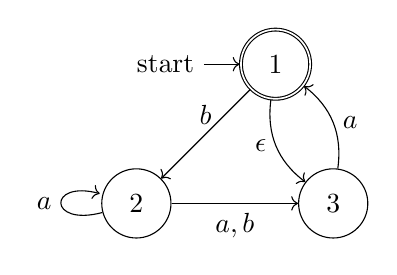
\begin{tikzpicture}[node distance = 25mm ]
    \node[state, initial, accepting] (1) {$1$};
    \node[state, below left of=1] (2) {$2$};
    \node[state, right of=2] (3) {$3$};

    \path[->] (1) edge[above] node{$b$} (2)
              (1) edge[below, bend right, left=0.3] node{$\epsilon$} (3)
              (2) edge[loop left] node{$a$} (2)
              (2) edge[below] node{$a, b$} (3)
              (3) edge[above, bend right, right=0.3] node{$a$} (1);
  \end{tikzpicture}
  \caption{An example NFA}
  \label{fig:NFA}
\end{figure}

Classically, a \emph{nondeterministic finite automaton} (NFA) is a finite state machine where
transitions are labeled with characters from a fixed alphabet $\Sigma$. These
are often represented formally as a 5-tuple $(Q, \Sigma, \delta, q_{0}, F)$,

\begin{itemize}
  \item $Q$ a finite set of states
  \item $\Sigma$ a fixed, finite alphabet
  \item $\delta : Q \times (\Sigma \cup \{ \varepsilon\}) \to \mathcal{P}(Q)$ the labeled transition function
  \item $q_{0} \in Q$ the start state
  \item $F \subset Q$ a set of accepting states
\end{itemize}

Intuitively, this can be thought of like a directed graph with nodes in $Q$ with
an edge $q \overset{c}{\to} q'$ whenever $q' \in \delta(q, c)$. Note that
transitions in an NFA may be labeled with the empty string $\varepsilon$ --- such
transitions are referred to as \emph{$\varepsilon$-transitions}. We may see an
example of an NFA in \cref{fig:NFA}.

From an NFA, we may construct a grammar of traces as follows:

First, we define a mutual fixed point grammar that describes the traces through the NFA.\ Then, we have another
grammar that tells us if we're currently in an accepting state of the automaton.
A parse of the NFA grammar is then a pair of a trace and the data that we're in
an accepting state.

Consider the NFA $N$ pictured in \cref{fig:NFA}. There are three states, $1$, $2$,
and $3$. We introduce a non-linear type $Q$ with three inhabitants $q_{1}$,
$q_{2}$, and $q_{3}$ to represent each of these states, respectively. Given a
$q, q'$, we can
then define the type of traces from $q$ to $q'$. For instance, let's construct
the traces starting at $q_{1}$ and ending at $q_{2}$ as an example.

\begin{equation}
  \label{eq:nfatrace}
  \mathsf{Trace}_{N}(q_{1}, q_{2}) = \mu
  \begin{pmatrix}
    g_{q_{1}} := g_{q_{3}} \oplus ( b \otimes g_{q_{2}} ) \\
    g_{q_{2}} := ( a \otimes g_{q_{2}} ) \oplus ( a \otimes g_{q_{3}} ) \oplus ( b \otimes g_{q_{3}} ) \oplus I \\
    g_{q_{3}} := a \otimes g_{q_{1}} \\
  \end{pmatrix}. g_{q_{1}}
\end{equation}

We should read this as defining three mutually recursive grammars, one for each
state. The definitions of these mutually recursive grammars capture the
transitions of the automaton. To ensure that we only encode traces that end in
state 2, we only include the unit $I$ as a summand in
$g_{q_{2}}$. That is, by only including $I$ at this location, it makes it the
only place where derivations of $\mathsf{Trace}(q_{1}, q_{2})$ can terminate. We
can think of all of these definitions underneath
of the $\mu$ binder as bringing some local grammars into scope. With these local
grammars in scope we are ultimately constructing a term of type $g_{q_{1}}$ to denote
only traces starting in state 1.

To encode the acceptance criteria of $N$, we want to internalize a proposition
over each state of the NFA.\ That is, for each $q \in Q$ we define a term

\[
  \mathsf{acc}(q) := q \text{ is accepting}
\]

In this example, $\mathsf{acc}(q_{1}) = \top$ and
$\mathsf{acc}(q_{2}) = \mathsf{acc}(q_{3}) = \bot$. An accepting trace of the NFA $N$ is then given by the following dependent grammar,
\[
 \mathsf{AccTrace}_{N} := \LinSigTy q Q {\left( \mathsf{Trace}_{N}(q_{0} , q) \amp \mathsf{acc}(q) \right)}
\]

where $q_{0}$ is the initial state. That is, a trace is accepted by the NFA if
we can construct the trace, and the trace ends at an accepting state. This idea
is simple enough and aligns with how we intuitively treat these automata.

Generalizing over the above example, we want to define the type of traces as,

\[
  \mathsf{Trace}_{N}(q_{0}, q_{1}) = \mu
  \begin{pmatrix}
    g_{q} := \mathsf{Trans}(q), & q \neq q_{1} \\
    g_{q} := \mathsf{Trans}(q) \oplus I , & q = q_{1}
  \end{pmatrix}. g_{q_{0}}
\]

where $\mathsf{Trans}(q)$ is an iterated disjunction that describes which
transition you should take. For an NFA, $\mathsf{Trans}(q)$ must take on the
following syntactic form,

\begin{gather*}
 \mathsf{State} \in \{ g_{q} : q \in Q \} \\
 \mathsf{Char} \in \Sigma \\
 \mathsf{Trans}_{N}(q) ::= \mathsf{Char} \otimes \mathsf{State}~|~\mathsf{State}~|~\mathsf{Trans}_{N}(q) \oplus \mathsf{Trans}_{N}(q)
\end{gather*}

That is, $\mathsf{Trans}(q)$ is a disjunction of literals followed by grammars
that encode states.

When conducting proofs involving NFA grammars, we often to
need either construct terms of type $\mathsf{Trace}_{N}(q , q')$. To
this end, we give three admissible rules for constructing
traces,

\begin{figure}[h!]
  \label{fig:admissibleintro}
  \begin{mathpar}
    \inferrule
    {~}
    {\Gamma ; \cdot \vdash \mathsf{nil} : \mathsf{Trace}_N
      (q , q)}

    \and

    \inferrule
    {\Gamma ; \Delta \vdash M : \mathsf{Trace}_N
      (dst , q') \\
    \exists \text{ transition } src \overset{c}{\to} dst
    }
    {\Gamma ; x : c , \Delta \vdash \mathsf{cons}(M) : \mathsf{Trace}_N
    (src , q')}

    \and

    \inferrule
    {\Gamma ; \Delta \vdash M : \mathsf{Trace}_N (dst , q')
      \\
    \exists~\varepsilon\text{-transition } src
    \overset{\varepsilon}{\to} dst}
    {\Gamma ; \Delta \vdash \mathsf{\varepsilon cons}(M) : \mathsf{Trace}_N
    (src , q')}
  \end{mathpar}
  \caption{Admissible Trace Constructors}
\end{figure}

That is, we may use $\mathsf{nil}$ to terminate a trace that
begins and ends at state $q$. The rules $\mathsf{cons}$ and
$\mathsf{\varepsilon cons}$ are then used to inductively
stitch traces together when sound. For instance, we can read
the $\mathsf{cons}$ rule as saying that we can
create a trace coming from a state $src$ provided that we may first
transition via the character $c$ to state $dst$ and
inductively build a trace starting from $dst$. The
$\mathsf{\varepsilon cons}$ rule says something similar, but
with an $\varepsilon$-transition instead of a transition
labelled by a character. Recall that
these rules are \emph{admissible}. They are not strictly
necessary as primitives to conduct our proofs; however, they
do provide convenient shorthand notation for building terms
of type $\mathsf{Trace}_{N}(q , q')$.

Dual to constructing traces, we often want to construct
other terms in a context containing values of type
$\mathsf{Trace}_{N}(q , q')$. For this purpose, we make use
of the elimination principle for multiple-fixed points ---
which we write as $\mathsf{mfold}$ --- given
in \cref{subsubsec:other}.

Note that this general construction will readily generalize to other types of
automata. If we wanted to define say deterministic finite automata\footnote{DFAs
\emph{could} just be defined as NFAs that happen to be deterministic. This is
one way to do so, or you may choose to present the transition relation for the
automaton as a transition \emph{function} instead. Concerns like these don't
matter so much when defining things on paper, but at formalization time these
are important and can make some proofs much easier.}, pushdown automata, Turing
machines, etc, we just swap out the type of traces for a different, but very
similar, trace construction.

With this setting for finite automata, we can now internalize some classical theorems inside of our formal system.


\subsection{A DFA Parser}
\label{subsec:regexparser}

Just as we encoded traces of NFAs as grammars, we likewise
encode the traces of a DFA as grammars. The key difference
between NFAs and DFAs is \emph{determinism} --- meaning,
that in a state $q$ inside of DFA, given a character $c$ there
will be exactly one transition that we may take leaving $q$
with label $c$. For us, this changes the definition of valid
transitions for a DFA, instead of the definition of
$\mathsf{Trans}$ provided in \cref{subsec:finiteaut} DFAs
obey

\begin{gather*}
 \mathsf{State} \in \{ g_{q} : q \in Q \} \\
 \mathsf{Trans}(q) ::= \bigoplus_{c \in \Sigma} (c \otimes \mathsf{State})
\end{gather*}

Meaning, each state has a transition for every character.

We now wish to define a parser term for DFA grammars. In
particular, for a DFA $D$ we want to build a term,

\[
  w : \String \vdash \mathsf{parse}_{D} : \mathsf{AccTrace}_{D} \oplus \top
\]

where left injection into the output type denotes acceptance
by the parser, and right injection denotes rejection. To
build such a parser, it will suffice to construct a term

\[
  w : \String \vdash \mathsf{parse}_{D} : \LinSigTy q Q {\mathsf{Trace}_{D}(q_{0} , q)}
\]
This is because given a trace of a DFA, we may easily check
if we should accept or reject by simply testing
if the final state is accepting.

Because $w$ is a Kleene star of characters, we may construct
our desired $\mathsf{parse}_{D}$ term as a $\mathsf{foldl}$
over $w$. In the empty case, we just have the trace that
ends at the accepting state. In the recursive case, we
effectively add to our trace by transitioning one character
at a time, as we read them moving across $w$.

\todoin{Derivation tree for this construction}

Perhaps this derivation is not too surprising. All it says
is that a DFA may be ran by transitioning a single character
at a time, and then accepting or rejecting based on the
final state. This is exactly what DFAs did initially, so
what did we gain? Well, this has the benefit of our type
system to ensure its correctness. Moreover, this construction exports to an
intrinsically verified and executable DFA via Agda.


\subsection{Regular Grammars and DFAs}
\label{subsec:deriv}

In order to extend the DFA
parser from \cref{subsec:regexparser} to the construction of
a verified parser
generator for regular grammars we need to perform some
plumbing establishing an equivalence between regular
expressions and DFAs.

There are several routes we may hope to take in establishing
this equivalence. First, we could prove an equivalence
between NFAs and regular expressions, and separately prove
an equivalence between NFAs and DFAs.
In \cref{subsec:eqproofs}, we include a version of
Thompson's construction --- which established the
equivalence between regular grammars and DFAs. We may additionally
hope to internalize a variant of the powerset construction \cite{rabinFiniteAutomataTheir1959}
--- which takes as input an NFA and constructs a DFA that
recognizes the same language --- and combine the results of
Thompson's construction and the powerset constructions to give an equivalence
between regular expressions and DFAs.  This route is alluring, as it
internalizes several classic grammar-theoretic constructions. However, it may
necessitate extensions to the LNL theory, like
a propositional truncation, and we have not yet investigated
how this would interact with the existing types in the
theory. The addition of a propositional truncation may seem
harmless, but it is not always immediately clear how
distinct constructions will interact. For instance, when
exploring LNL models, Benton discovered that the synthesis
of linear and dependent types require a new presentation of
the $!$ modality from linear logic
\cite{bentonMixedLinearNonlinear1995}. That is all to say,
this is a work in progress and
it is not immediate that the addition of a propositional
truncation is adequate for establishing the weak equivalence
between NFAs and DFAs.

We may instead hope to internalize an equivalence between
regular grammars and DFAs by using Brzozowski derivatives to
directly create a DFA that is weakly equivalent to a given
regular expression, as described by Owens et al.
\cite{owensRegularexpressionDerivativesReexamined2009}.
One characterization of regular grammars is that they are
precisely those grammars which have finitely many inequivalent Brzozowski
derivatives
\cite{brzozowskiDerivativesRegularExpressions1964}.
The algorithm used by Owens takes in a
regular grammar and generates a DFA that recognizes the same
language, and the states in this DFA are the finitely many
derivative equivalence classes. We initially had a version of
this theorem very roughly internalized in the LNL theory.
To our taste, too much of this presentation relied on
meta-arguments that lived outside of
our formalism, and thus this particular phrasing of the
theorem did not translate well into formalization.

In any case, we believe
that revisiting these lines of thought will lead to a
satisfactory internalization of the equivalence between
regular grammars and DFAs, and thus would bridge the gap
between our DFA parser and a full regular expression parser.

\subsection{Equivalence Between Regular Grammars and Finite Automata}
\label{subsec:eqproofs}
In this section, we describe a version of Thompson's
construction \cite{thompsonProgrammingTechniquesRegular1968}
   where we construct an NFA that recognizes a given regular
expression. Moreover, we will show that this NFA is strongly equivalent to the
original grammar. Witnessing this construction in our syntax has two benefits
\begin{enumerate}
  \item It reinforces this high-level view that the syntax is a natural and
        general setting for formal grammar reasoning, as we demonstrate that
        this formal system subsume results from existing systems, and
  \item Following the
        development of Thompson's construction, we then need
        only establish the equivalence of NFAs and DFAs to
        complete the full regular expression parser
\end{enumerate}

\begin{theorem}[Thompson]
  \label{thm:thompson}
  For $g$ a regular grammar $g$, there is an NFA $N$ that recognizes the same
  language as $g$.
\end{theorem}

We make a pretty straightforward adaptation of Thompson's theorem to our setting,

\begin{theorem}[Typed Thompson]
  \label{thm:typthompson}
  For $g$ a regular grammar $g$, there is an NFA $N$ such that $g$ is isomorphic
  to $\mathsf{AccTrace}_{N}$.
\end{theorem}

\begin{proof}[Proof Sketch]
  The following proof is currently formalized in Agda. Below
  we give a walk through the structure of the proof.

  Recall that regular grammars are inductively defined via
  disjunction, concatenation, and Kleene star over literals
  and the empty grammar. By induction over regular grammars,
  we will construct an NFA that is equivalent to $g$.

  First, define the recognizing NFA for the empty grammar
  $I$.

  \begin{figure}[h!]
  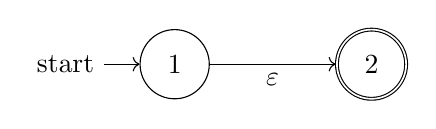
\begin{tikzpicture}[node distance = 25mm ]
    \node[state, initial] (1) {$1$};
    \node[state, right of=1, accepting] (2) {$2$};

    \path[->] (1) edge[below] node{$\varepsilon$} (2);
  \end{tikzpicture}
  \caption{$NFA(I)$}
  \label{fig:emptyNFA}
  \end{figure}

  The type of traces from the initial state of $NFA(I)$ to the single
  accepting state is given by,

  \[
    \mathsf{Trace}_{NFA(I)}(q_{1}, q_{2}) = \mu
      \begin{pmatrix}
         g_{q_{1}} := g_{q_{2}} \\
         g_{q_{2}} := I
      \end{pmatrix}. g_{q_{1}}
  \]

  The accepting traces through $NFA(I)$ are then described
  as,

  \[
    \mathsf{AccTrace}_{NFA(I)} = \LinSigTy q {\{1 , 2\}} {\left( \mathsf{Trace}_{NFA(I)}(q_{1} , q) \amp \mathsf{acc}(q) \right)}
  \]

  A quick inspection of \cref{fig:emptyNFA} reveals that the
  only reasonable choice for $q$ is $q_{2}$ --- because
  state 2 is accepting while state 1 is not. Therefore,

  \begin{align*}
    \mathsf{AccTrace}_{NFA(I)}
    & \cong \mathsf{Trace}_{NFA(I)}(q_{1} , q_{2}) \amp \mathsf{acc}(q_{2}) \\
    & \cong \mathsf{Trace}_{NFA(I)}(q_{1} , q_{2}) \amp \top \\
    & \cong \mathsf{Trace}_{NFA(I)}(q_{1} , q_{2})
  \end{align*}

  From here, to prove
  $I \cong \mathsf{AccTrace}_{NFA(I)}$ it suffices to show
  $I \cong \mathsf{Trace}_{NFA(I)}(q_{1} , q_{2})$. Below we
  give two parse transformers, one from $I$ to
  $\mathsf{Trace}_{NFA(I)}(q_{1} , q_{2})$ and vice versa. The formalized
  artifact provides the low-level details that these are
  indeed mutually inverse.

  \[
    \inferrule
    {p : I \vdash \mathsf{nil} : \mathsf{Trace}(q_{2} , q_{2}) \\
     \exists \text{~transition~} q_{1} \overset{\varepsilon}{\to} q_{2}
    }
    {p : I \vdash \mathsf{\varepsilon cons}(\mathsf{nil}) : \mathsf{Trace}_{NFA(I)}(q_{1} , q_{2})}
  \]

  Let $\gamma$ be the substitution $\{ g_{q_{2}} / g_{q_{1}}, I / g_{q_{2}} \}$,

  \[
    \inferrule
    {
      p : \mathsf{Trace}_{NFA(I)}(q_{1} , q_{2}) \vdash p :
        \mathsf{Trace}_{NFA(I)}(q_{1} , q_{2}) \\
      x_{1} : \simulsubst {g_{q_{2}}} {\gamma} = I \vdash x_{1} : I \\
      x_{2} : \simulsubst {I} {\gamma} = I \vdash x_{2} : I
    }
    {
      p : \mathsf{Trace}_{NFA(I)}(q_{1} , q_{2}) \vdash \mathsf{mfold}(x_{1}.x_{1} , x_{2}.x_{2})(p) : I
    }
  \]

  This concludes the proof for the case of the empty
  grammar. Let's now walk through the construction for
  literal grammars. Given a character $c$, we construct an
  NFA that recognizes only the string containing the single
  character $c$ as,


  \begin{figure}[h!]
  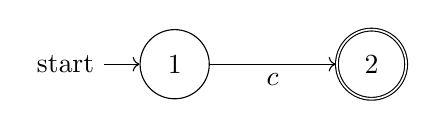
\begin{tikzpicture}[node distance = 25mm ]
    \node[state, initial] (1) {$1$};
    \node[state, right of=1, accepting] (2) {$2$};

    \path[->] (1) edge[below] node{$c$} (2);
  \end{tikzpicture}
  \caption{$NFA(c)$}
  \label{fig:literalNFA}
  \end{figure}

  The automaton in \cref{fig:literalNFA} induces the
  following type of traces from $q_{1}$ to $q_{2}$.

  \[
    \mathsf{Trace}_{NFA(c)}(q_{1}, q_{2}) = \mu
      \begin{pmatrix}
         g_{q_{1}} := c \otimes g_{q_{2}} \\
         g_{q_{2}} := I
      \end{pmatrix}. g_{q_{1}}
  \]

  Through the same argument as the empty grammar, the only
  state that is accepting is $q_{2}$ and thus,

  \[
    \mathsf{AccTrace}_{NFA(c)} \cong \mathsf{Trace}_{NFA(c)}(q_{1} , q_{2})
  \]

  To show the desired isomorphism of $c \cong NFA(c)$ we
  make a similar argument as we did for the empty grammar
  $I$, except we leverage the $\mathsf{cons}$ rule instead
  of $\mathsf{\varepsilon cons}$. That is, the parse
  transformers in either direction are given as,

  \[
    \inferrule
    {\cdot \vdash \mathsf{nil} : \mathsf{Trace}(q_{2} , q_{2}) \\
     \exists \text{~transition~} q_{1} \overset{c}{\to} q_{2}
    }
    {p : c \vdash \mathsf{cons}(\mathsf{nil}) :
      \mathsf{Trace}_{NFA(c)}(q_{1} , q_{2})}
  \]


  \[
    \inferrule
    {
      p : \mathsf{Trace}_{NFA(c)}(q_{1} , q_{2}) \vdash p :
        \mathsf{Trace}_{NFA(c)}(q_{1} , q_{2}) \\
      x_{1} : \simulsubst {(c \otimes g_{q_{2}})} {\gamma} = c \otimes I \vdash \mathsf{unitR}(x_{1}) : c \\
      x_{2} : \simulsubst {I} {\gamma} = I \vdash x_{2} : I
    }
    {
      p : \mathsf{Trace}_{NFA(c)}(q_{1} , q_{2}) \vdash \mathsf{mfold}(x_{1}.\mathsf{unitR}(x_{1}) , x_{2}.x_{2})(p) : c
    }
  \]

  Where $\gamma$ is the substitution
  $\{ c \otimes g_{q_{2}} / g_{q_{1}}, I / g_{q_{2}} \}$ and
  $\mathsf{unitR}$ is a witness to the isomorphism
  $c \otimes I \cong c$. Again, we may see that these do
  indeed mutually invert each other in the Agda code.

  It remains to show that the desired isomorphisms are
  preserved by $\otimes$, $\oplus$, and Kleene star. Here,
  we will give the argument for the disjunction case, the
  others are defined quite similarly.

  Given two NFAs $N$ and $M$, we may define a new NFA that
  encodes the disjunction of $N$ and $M$. Denote the
  internal states of $N$ by $q_{j}$'s and the internal states
  of $M$ by $r_{k}$'s,

  \begin{figure}[h!]
  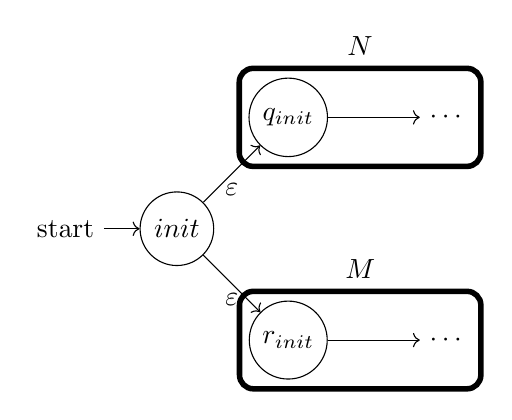
\begin{tikzpicture}[node distance = 20mm ]
    \node[state] (2) {$q_{init}$};
    \node[state, initial, below left of=2] (1) {$init$};
    \node[state, below right of=1] (3) {$r_{init}$};
    \node[right of=2] (4) {$\cdots$};
    \node[right of=3] (5) {$\cdots$};
    % \node[state, below right of=1] (3) {$3$};
    % \node[state, below of=2] (4) {$4$};

    \path[->] (1) edge[below] node{$\varepsilon$} (2);
    \path[->] (1) edge[below] node{$\varepsilon$} (3);
    \path[->] (2) edge[below] node{} (4);
    \path[->] (3) edge[below] node{} (5);

    \node[label={[name=l] $N$}, draw,line width=2pt,rounded corners=5pt, fit=(2)(4)] {};
    \node[label={[name=l] $M$}, draw,line width=2pt,rounded corners=5pt, fit=(3)(5)] {};
  \end{tikzpicture}
  \caption{$N \oplus_{NFA} M$}
  \label{fig:disjunctionNFA}
  \end{figure}

  \cref{fig:disjunctionNFA} shows the process of
  disjunctively combining NFAs. Precisely, we add a single
  new state and we included copies of the states from each of $N$
  and $M$. The new state acts as the initial state and has
  $\varepsilon$-transitions to the initial states of $N$ and
  $M$. We include all of the internal transitions from $N$
  and $M$, and the accepting states of $N \oplus_{NFA} M$
  are exactly the accepting states in each subautomaton.

  Let $g$ and $g'$ be two regular grammars such that
  $g \cong NFA(g)$ and $g' \cong NFA(g')$. As a matter of
  notation\footnote{We shall similarly abuse notation for
    $\otimes$ and Kleene. That is, for a regular grammar
    $g$, when we write $NFA(g)$ we mean the NFA inductively
    built up with the NFA-analogues to the constructors that
    built up $g$.}, we will write $NFA(g \oplus g')$ for
  $NFA(g) \oplus_{NFA} NFA(g')$. The traces of
  $NFA(g \oplus g')$ are then given by,

  \[
    \mathsf{Trace}_{NFA(g \oplus g')}(src , dst) = \mu
      \begin{pmatrix}
        g_{init} := g_{q_{0}} \oplus g_{r_{0}} \\
        g_{q_{j}} := \mathsf{Trans}_{NFA(g)}(q_{j}) \oplus \mathsf{isDst}(q_{j}) \\
        g_{r_{k}} := \mathsf{Trans}_{NFA(g')}(r_{k}) \oplus \mathsf{isDst}(r_{k})
      \end{pmatrix}.g_{src}
    \]

  where $\mathsf{Trans}$ is used to echo the same syntactic
  definitions that appear in the $NFA(g)$ and $NFA(g')$.
  Also, $src$ and $dst$ may take on any value in
  $Q := \{init\} \cup \{q_{j}\} \cup \{r_{k}\}$, and
  $\mathsf{isDst}(q)$ checks if $q$ is equal to $dst$. Which
  is all to say, the traces of $NFA(g \oplus g')$ comprise
  either a trace of $NFA(g)$, or a trace of $NFA(g')$, and
  the transition coming out of $g_{init}$ determines which
  subautomaton we step into.

  The parse transformer from $g \oplus g'$ checks which side
  of the sum type we are on, then takes the appropriate step
  from $g_{init}$ in the automaton.

  \[
    \inferrule
    {
      u : g \vdash \iota (\phi (u)) : \mathsf{AccTrace}_{NFA(g \oplus g')} \\
      v : g' \vdash \iota' (\psi (v)) : \mathsf{AccTrace}_{NFA(g \oplus g')}
    }
    {p : g \oplus g' \vdash \mathsf{case}~p \{ \mathsf{inl}(u) \mapsto s , \mathsf{inr}(v) \mapsto r \} : \mathsf{AccTrace}_{NFA(g \oplus g')}}
  \]

  with $\iota$ and $\iota'$ as embeddings from $NFA(g)$ and
  $NFA(g')$, respectively, into $NFA(g \oplus g')$,
  $\phi: g \cong \mathsf{AccTrace}_{NFA(g)}$, and $\psi: g' \cong \mathsf{AccTrace}_{NFA(g')}$. On a
  high level, all this construction does is turn a parse of
  $g$ into a parse of $NFA(g)$ and then embeds that inside
  of the larger automaton $NFA(g \oplus g')$. Likewise for $g'$.

  In the other direction, recall that the data of an
  accepting trace for $NFA(g \oplus g')$ is a pair of a
  trace and a proof that
  the end state $q'$ of that trace is accepting. By
  multifolding over the first part of that pair, we turn the
  term of type
  $\mathsf{Trace}_{NFA(g \oplus g')}(init , q')$ into a
  trace of either of the subautomata,

  \[
    p : \mathsf{Trace}_{NFA(g \oplus g')}(init , q') \vdash \mathsf{mfold}_{NFA(g \oplus g')} : \mathsf{Trace}_{NFA(g)}(q_{0} , q') \oplus \mathsf{Trace}_{NFA(g')}(r_{0} , q')
  \]

  Additionally, we leverage the fact that the only accepting
  states for $NFA(g \oplus g')$ are those from the
  subautomata to extract that $q'$ must be an accepting
  state from a subautomaton.

  \[
    x : \mathsf{acc}_{NFA(g \oplus g')}(q') \vdash M : \mathsf{acc}_{NFA(g)}(q') \oplus \mathsf{acc}_{NFA(g')}(q')
  \]

  We then combine the trace and proof of acceptance into an
  accepting trace of one of the subautomata,

  \[
    p : \mathsf{AccTrace}_{NFA(g \oplus g')} \vdash N : \mathsf{AccTrace}_{NFA(g)} \oplus \mathsf{AccTrace}_{NFA(g')}
  \]

  Lastly, we then inductively use the isomorphisms $\phi$
  and $\psi$ to turn the accepting traces into a parse of
  $g$ or $g'$,

  \[
     N : \mathsf{AccTrace}_{NFA(g)} \oplus \mathsf{AccTrace}_{NFA(g')} \vdash \mathsf{case}~N~\{\mathsf{inl}(n) \mapsto \phi^{-1}(n), \mathsf{inr}(n') \mapsto \psi^{-1}(n')\} : g \oplus g'
  \]

  As discussed above, the other cases and low-level details
  of isomorphism are reserved for the formalization. This
  concludes the proof of our variant of Thompson's construction.
\end{proof}

\subsection{Other Automata}
\subsubsection{Pushdown Automata}
\label{subsubsec:pda}
A (nondeterministic) \emph{pushdown automaton} is an automaton that employs a
stack. Just like NFAs, they have transitions labeled with characters from a
fixed string alphabet $\Sigma$. Additionally, they maintain a stack of
characters drawn from a stack alphabet $\Gamma$. They are often represented
formally as a 7-tuple $(Q, \Sigma, \Gamma, \delta, q_{0}, Z, F)$,

\begin{itemize}
  \item $Q$ a finite set of states
  \item $\Sigma$ a fixed, finite string alphabet
  \item $S$ a fixed, finite stack alphabet
  \item
        $\delta \subset Q \times (\Sigma \cup \{ \varepsilon \}) \times S \to \mathcal{P}(Q \times S^{*})$
        the transition function
  \item $q_{0} \in Q$ the start state
  \item $Z \in S$ the initial stack symbol
  \item $F \subset Q$ the accepting states
\end{itemize}

We encode the traces of a pushdown automaton very similarly to those of an NFA,
except the transitions of a PDA are instead encoded via the linear-non-linear
$\Pi$-type. This is because of simply transitioning via character, a PDA must
also pop and push characters onto a stack, which is used as the argument to
these dependent functions.

Let $S$ be a non-linear type encoding the stack
alphabet, and build lists over $S$ as the (non-linear) least fixed-point
$\mathsf{List}(S) := \mu X . 1 + S \times X$. Then, the type of states for a
PDA $P$ with stack alphabet $S$ are given as a functions that takes in lists $L$,
and then makes a case distinction between possible transitions based on what was witnessed as $\mathsf{head}(L)$. The choice of transition
will then determine which character to transition by and what word $w$ should be
pushed onto the stack. The word that is added to the top of the stack is
appended to $\mathsf{tail}(L)$ and then we recursively step into another state
called on argument $w + \mathsf{tail}(L)$.

% \begin{gather*}
%   \mathsf{State} \in {g _{q} : q \in Q} \\
%   \mathsf{Word} \in \String \\
%   \mathsf{Char} \in \Sigma   \\
%   \mathsf{StackChar} \in \Gamma \\
% \end{gather*}
% \begin{align*}
%   \mathsf{Trans}_{P}(q) ::=~&
%                            \LinPiTy {(hd :: tl)} {\mathsf{List}(S)} {\left( \mathsf{Char} \otimes \mathsf{State}(\mathsf{Word} + tl) \right)}~| \\
%   & \LinPiTy {(hd :: tl)} {\mathsf{List}(S)} {\left(  \mathsf{State}(\mathsf{Word} + tl) \right)}~|~\mathsf{Trans}_{P}(q) \oplus \mathsf{Trans}_{P}(q)
% \end{align*}

% That is to say, when transitioning a PDA pops off the head $hd$ of the stack

\subsubsection{Turing Machines}
\label{subsubsec:tm}

In
\cref{subsubsec:pda}, we gave a grammar presentation of
traces through a PDA by using a non-linear type $S$
to encode the stack. We may similarly use pairs $S \times S$
to encode the tape of a Turing machine. With two stacks we can simulate the behavior of the
infinite tape of a Turing machine. The intuition behind this correspondence is
that the left half of the tape is on one stack, the right
half of the tape the other, and we treat the tops of stacks
like the head of the tape.

Due to computability limitations, we are not able to extract
a verified parser for all recursively enumerable languages.
Yet we should still reflect on the generality of our syntax,
as it allows a natural encoding of Turing machines.

\section{Future Work}
\label{sec:future}

\subsection{Implementation for Context-Free Grammars}
As suggested throughout the paper and briefly explored in
\cref{subsubsec:pda}, the first extension to the work in
this paper will be to bring analogous constructions to
context-free grammars and their accompanying pushdown automata.

\subsection{Beyond Strings}
\label{subsec:beyond}

While parsing typically refers to the generation of semantic
objects from string input, many tasks in programming can be
viewed as parsing of objects with more structure, such as
trees with binding structure or graphs. Fundamental to the
frontend of many
programming language implementations are type systems. In
particular, \emph{type checking}
--- analogous to language recognition --- and \emph{typed
  elaboration} --- analogous to parsing --- arise when
producing a semantic object subject to some analysis. Just
as our string grammars were given as functors from $\String$
to $\Set$, we envision adapting the same philosophy
to functors from $\String$ to \emph{trees} to craft a syntax
that natively captures typed elaboration. This suggests an
unusual sort of bunched type theory, where context extension
no longer resembles concatenation of strings but instead
takes on the form of tree constructors.

Thus far, our theory has proved useful for internalizing long-standing
grammar-theoretic constructions, but there has been decades of research
conducted since. A fruitful avenue for future work includes
testing if our formalism can also internalize more recently proposed grammar
mechanisms, such as the interval parsing grammars given by Zhang et al. \cite{zhangIntervalParsingGrammars2023}.

\newpage

\bibliographystyle{plain}
\bibliography{refs.bib}

\newpage

\appendix

\section{Inference Rules}
\label{sec:infer}

\begin{figure}[h!]
  \label{fig:structjdg}
  \begin{mathpar}
    \inferrule{~}{\ctxwff \cdot}
    \and
    \inferrule{\ctxwff \Gamma \\ \ctxwffjdg \Gamma X}{\ctxwff {\Gamma, x : X}}

    \\

    \inferrule{~}{\linctxwff \Gamma \cdot}
    \and
    \inferrule{\linctxwff \Gamma \Delta \\ \linctxwffjdg \gamma A}{\linctxwff \Gamma {\Delta, a : A}}

    \\

    \inferrule{\Gamma \vdash X : U_i}{\ctxwffjdg \Gamma X}

    \and

    \inferrule{\Gamma \vdash A : L_i}{\linctxwffjdg \Gamma A}

    \\

    \inferrule{\Gamma \vdash X \equiv Y : U_i}{\ctxwffjdg \Gamma {X\equiv Y}}

    \and

    \inferrule{\Gamma \vdash A \equiv B : L_i}{\linctxwffjdg \Gamma {A \equiv B}}

  \end{mathpar}
  \caption{Structural judgments}
\end{figure}

\begin{figure}
  \label{fig:typewf}
  \begin{mathpar}
    \inferrule{~}{\Gamma \vdash U_i : U_{i+1}}
 %
    \and
%
    \inferrule{~}{\Gamma \vdash L_i : U_{i+1}}
%
    \\
%
    \inferrule{\Gamma \vdash X : U_i \\ \hspace{-0.1cm} \Gamma, x : X \vdash Y : U_i}{\Gamma \vdash \PiTy x X Y : U_i }%
%
    \and
%
    \inferrule{\Gamma\vdash X : U_i \\ \hspace{-0.1cm} \Gamma, x : X \vdash Y : U_i}{\Gamma \vdash \SigTy x X Y : U_i}
%
    \\
%
    \inferrule{~}{\Gamma \vdash 1 : U_i}
%
    \and
%
    \inferrule{\Gamma \vdash A : L_i}{\Gamma \vdash G A : U_i}
%
    \\
%
    \inferrule{~}{\Gamma \vdash I : L_i}
 %
    \and
%
    \inferrule{\Gamma \vdash A : L_i \\ \hspace{-0.1cm}\Gamma \vdash B : L_i}{\Gamma \vdash A \otimes B : L_i}
%
    \and
%
    \inferrule{\Gamma \vdash A : L_i \\ \hspace{-0.1cm}\Gamma \vdash B : L_i}{\Gamma \vdash A \lto B : L_i}
%
    \and
%
    \inferrule{\Gamma \vdash A : L_i \\ \hspace{-0.1cm}\Gamma \vdash B : L_i}{\Gamma \vdash B \tol A : L_i}
%
    \\
%
    \inferrule{\Gamma \vdash X : U_i \\ \Gamma, x : X \vdash A : L_i}{\Gamma \vdash \LinPiTy x X A : L_i}
%
    \and
%
    \inferrule{\Gamma \vdash X : U_i \\ \Gamma, x : X \vdash A : L_i}{\Gamma \vdash \LinSigTy x X A : L_i}
%
    \\
%
    \inferrule{\Gamma \vdash X : U_i \quad \{\Gamma \vdash e_i : X\}_i}{\Gamma \vdash e_1 =_X e_2 : U_i}
    %
    \and
    %
    \inferrule{~}{\Gamma \vdash \top : L_i}
%
    \and
%
    \inferrule{\Gamma \vdash A : L_i \quad \Gamma \vdash B : L_i}{\Gamma \vdash A \amp B : L_i}
%
    \\
    %
    \inferrule{c \in \Sigma}{\Gamma \vdash c : L_0}
    %
    \and
    %
    \inferrule{\Gamma, x : L_i \vdash A : L_i \and A \textrm{ strictly positive}}{\Gamma \vdash \mu x.\, A : L_i}
  \end{mathpar}
  \caption{Type well-formedness}
\end{figure}

\begin{figure}
  \label{fig:jdgeq}
  \begin{mathpar}
    \inferrule{\Gamma \vdash p : e =_X e'}{\Gamma \vdash e \equiv e' : X}
%
    \and
%
    \inferrule{~}{\Gamma \vdash \app {(\lamb x e)} {e'} \equiv \subst x e {e'} : X}
%
    \and
%
    \inferrule{~}{\Gamma \vdash e \equiv \lamb x {\app e x} : \PiTy x X Y}
%
    \and
%
    \inferrule{~}{\Gamma \vdash \pi_1\, (e_1, e_2) \equiv e_1 : X}
%
    \and
%
    \inferrule{~}{\Gamma \vdash \pi_2\, (e_1, e_2) \equiv e_2 : \subst x {e_1} Y}
%
    \and
%
    \inferrule{~}{\Gamma \vdash e \equiv (\pi_1\, e, \pi_2\, e) : \SigTy x X Y}
%
    \and
%
    \inferrule{~}{}
%
    \inferrule{~}{\Gamma \vdash t \equiv t' : 1}
%
    \and
%
    \inferrule{~}{\Gamma \vdash G\, (G^{-1} \, t) \equiv t : G A}
%
    \and
%
    \inferrule{~}{\Gamma; \cdot \vdash G^{-1}\, (G \, t ) \equiv t: A}
%
    \and
%
    \inferrule{~}{\Gamma; \Delta \vdash \app {(\lamblto a e)} {e'} \equiv \subst e x {e'} : C}
%
    \and
%
    \inferrule{~}{\Gamma; \Delta \vdash e \equiv \lamblto a {\app e a} : A \lto B}
%
    \and
%
    \inferrule{~}{\Gamma; \Delta \vdash \app {(\lambtol a e)} {e'} \equiv \subst e x {e'} : C}
%
    \and
%
    \inferrule{~}{\Gamma; \Delta \vdash e \equiv \lambtol a {\app e a} : A \tol B}
%
    \and
%
    \inferrule{~}{\Gamma; \Delta \vdash \app {(\dlamb x e)} {e'} \equiv \subst x a {e'} : C}
%
    \and
%
    \inferrule{~}{\Gamma; \Delta \vdash e \equiv \dlamb x {\app e x} : \LinPiTy x X A}
%
    \and
%
    \inferrule{~}{\Gamma; \Delta \vdash e \equiv e' : \top}
%
    \and
%
    \inferrule{~}{\Gamma; \Delta \vdash e_i \equiv \pi_i (e_1, e_2) : A_i}
%
    \and
%
    \inferrule{~}{\Gamma; \Delta \vdash e \equiv (\pi_1 e, \pi_2 e) : A\& B}
%
    \and
%
    \inferrule{~}{\Gamma; \Delta \vdash \letin {()} {()} e \equiv e : C}
    %
    \and
    %
    \inferrule{~}{\Gamma; \Delta \vdash \letin {()} e {\subst {e'} {()} a} \equiv \subst {e'} a e : C}
%
    \and
%
    \inferrule{~}{\Gamma; \Delta \vdash \letin {e \otimes e'} {a \otimes a'} e'' \equiv \subst {e''} {a, a'} {e, e'} : C}
%
    \and
    %
    \inferrule{~}{\Gamma; \Delta \vdash \letin {a \otimes b} e {\subst {e'} {a \otimes b} c} \equiv \subst {e'} c e : C}
%
    \and
%
    \inferrule{~}{\Gamma;\Delta \vdash \letin {(x, a)} {(e, e')} {e''} \equiv \subst {e''} {x, a} {e, e'} : C}
    %
    \and
    %
    \inferrule{~}{\Gamma; \Delta \vdash \letin {(x, a)} e {\subst {e'} {(x, a)} y} \equiv \subst {e'} e y : C}
\end{mathpar}
  \caption{Judgmental equality}
\end{figure}

\begin{figure}
  \label{fig:inttyping}
  \begin{mathpar}
  \inferrule{~}{\Gamma, x : X, \Gamma' \vdash x : X}
  %
  \and
  %
  \inferrule{\Gamma \vdash e : Y \quad \ctxwffjdg \Gamma {X \equiv Y}}{\Gamma \vdash e : X}
  %
  \\\
  %
  \inferrule{~}{\Gamma \vdash () : 1}
  %
  \and
  %
  \inferrule{\Gamma \vdash e : X \\ \Gamma \vdash e : \subst Y e x}{\Gamma \vdash (e, e') : \SigTy x X Y}
  %
  \\
%
  \inferrule{\Gamma \vdash e : \SigTy x X Y}{\Gamma \vdash \pi_1\, e : X}
  %
  \and
  %
  \inferrule{\Gamma \vdash e : \SigTy x X Y}{\Gamma \vdash \pi_2\, e : \subst Y {\pi_1\, e} x}
  \and
  \inferrule{\Gamma, x : X \vdash e : Y}{\Gamma \vdash \lamb x e : \PiTy x X Y}
  %
  \and
  %
  \inferrule{\Gamma \vdash e : \PiTy x X Y \\ \Gamma \vdash e' : X}{\Gamma \vdash \app e {e'} : \subst Y {e'} x}
  %
  \\
  %
  \inferrule{\Gamma \vdash e \equiv e' : X}{\Gamma \vdash \mathsf{refl} : e =_X e'}
  \and
  \inferrule{\Gamma ; \cdot \vdash e : A}{\Gamma \vdash \mathsf G e : \mathsf G A}
  \end{mathpar}
  \caption{Intuitionistic typing}
\end{figure}

\begin{figure}
  \label{fig:linsyntax}
  \begin{mathpar}
    \inferrule{~}{\Gamma ; a : A \vdash a : A}
    \and
    \inferrule{\Gamma ; \Delta \vdash e : B \\ \linctxwffjdg \Gamma {A \equiv B}}{\Gamma ; \Delta \vdash e : A}
    %
    \\
    %
    \inferrule{~}{\Gamma ; \cdot \vdash () : I}
    \and
    \inferrule{\Gamma ; \Delta \vdash e : I \\ \Gamma ; \Delta_1',\Delta_2' \vdash e' : C}{\Gamma ; \Delta_1',\Delta,\Delta_2' \vdash \letin {()} e {e'} : C}
    %
    \\
    %
    \inferrule{\Gamma ; \Delta \vdash e : A \\ \Gamma ; \Delta' \vdash e' : B}{\Gamma ; \Delta, \Delta' \vdash e \otimes e' : A \otimes B}
    %
    \\
    %
    \inferrule{\Gamma ; \Delta \vdash e : A \otimes B \\ \Gamma ; \Delta'_1, a : A, b : B, \Delta'_2 \vdash e'}{\Gamma ;  \Delta_1', \Delta, \Delta'_2 \vdash \letin {a \otimes b} e {e'}}
    \\
    %
    \inferrule{\Gamma ; a : A , \Delta \vdash e : B}{\Gamma ; \Delta \vdash \lamblto a e : A\lto B}
    \and
    \inferrule{\Gamma ; \Delta' \vdash e' : A \\ \Gamma ; \Delta \vdash e : A \lto B}{\Gamma ; \Delta', \Delta \vdash \applto {e'} {e} : B}
    \\
    %
    \inferrule{\Gamma ; \Delta , a : A \vdash e : B}{\Gamma ; \Delta \vdash \lambtol a e : B\tol A}
    \and
    \inferrule{\Gamma ; \Delta \vdash e : B \tol A \\ \Gamma ; \Delta' \vdash e' : A}{\Gamma ; \Delta, \Delta' \vdash \apptol e {e'} : B}
    %
    \\
    %
    \inferrule{\Gamma, x : X ; \Delta  \vdash e : A}{\Gamma ; \Delta \vdash \dlamb x e : \LinPiTy x X A}
    \and
    \inferrule{\Gamma ; \Delta \vdash e : \LinPiTy x X A \\ \Gamma \vdash e' : X}{\Gamma ; \Delta \vdash \app e {e'} : \subst A {e'} x}
    %
    \\
    %
    \inferrule{\Gamma \vdash e : X \quad \Gamma ; \Delta \vdash e' : \subst A e x}{\Gamma ; \Delta \vdash (e, e') : \LinSigTy x X A}
    %
    \\
    %
    \inferrule{\Gamma ; \Delta \vdash e : \LinSigTy x X A \quad \Gamma, x : X ; \Delta'_1, a : A, \Delta'_2 \vdash e' : C}{\Gamma; \Delta'_1, \Delta, \Delta'_2 \vdash \letin {(x, a)} e {e'}: C}
    %
    \\
    %
    \inferrule{~}{\Gamma ; \Delta \vdash () : \top}
    %
    \\
    %
    \inferrule{\Gamma ; \Delta \vdash e_1 : A_1 \quad \Gamma ; \Delta \vdash e_2 : A_2}{\Gamma ; \Delta \vdash (e_1, e_2) : A_1 \amp A_2}
    \and
    \inferrule{\Gamma ; \Delta \vdash e : A_1 \amp A_2 }{\Gamma ; \Delta \vdash \pi_i \, e : A_i}
    %
    \\
    %
    \inferrule{\Gamma \vdash e : \mathsf{G} A}{\Gamma ; \cdot \vdash \mathsf{G}^{-1}\, e : A}
    %
    \\
    %
    \inferrule{\Gamma; \Delta \vdash e : \subst A {\mu x.\, A} x}{\Gamma; \Delta \vdash \mathsf{cons}\, e : \mu x.\, A}
    \and
    \inferrule{\Gamma;\Delta\vdash e' : \mu x.\,A \and \Gamma; a:\subst A B x \vdash e : B}{\Gamma;\Delta\vdash \mathsf{fold}(a.e)(e') : B}
  \end{mathpar}
  \caption{Linear typing}
\end{figure}
\end{document}
